The Butler framework has been built to enable large-scale scientific analyses in the cloud and the largest set of analyses that have been performed using this framework to date have been the Germline analyses for the Pan-Cancer Analysis of Whole Genomes Project on the EBI Embassy Cloud. We describe the nature of these analyses as well as the details of the Butler deployment on the Embassy Cloud next.

\section{Deployment on EMBL/EBI Embassy Cloud}

The EMBL/EBI Embassy Cloud\autocite{cook2016european} is an academic cloud computing center which runs an Openstack-based environment. The Embassy Cloud plays a key role in the PCAWG project by donating substantial storage and cloud computing capacity over the course of 3 years. The total amount of resources dedicated to the project by the Embassy Cloud is:

\begin{itemize}
\item 1 PB Isilon storage shared over NFS
\item 1500 compute cores
\item 6 TB RAM
\item 40 TB local SSD storage
\item 10 Gb network
\end{itemize}

These resources have been used to host one of the seven PCAWG GNOS repositories that exist worldwide, as well as performing a number of scientific analyses for the project. We have used Butler extensively on the Embassy Cloud in order to carry out the germline analyses for PCAWG-8 Working Group.

\begin{figure}[H]
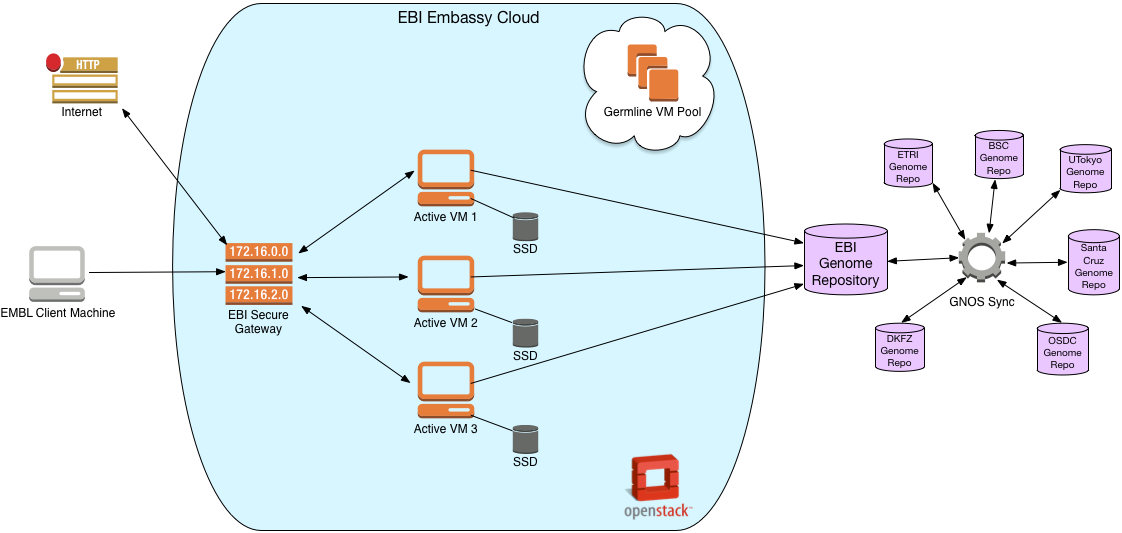
\includegraphics[width=\textwidth]{embassy_architecture}
\centering
\caption {Embassy Cloud Architecture}
\label{fig:embassy_architecture}
\end{figure}

\subsubsection{Embassy Cloud Architecture}

Figure \ref{fig:embassy_architecture} shows the general high-level architecture of the Germline Working Group's tenant within the EMBL/EBI's Embassy Cloud. Because of the sensitive nature of the genetic data that is stored at Embassy there are several security mechanisms in place. The Virtual Machines are hidden behind a secure gateway and are not visible to the external network. The secure gateway maintains a hand-curated list of IP addresses that are allowed to connect to it from the Internet. Currently this list contains several IP addresses of research institutions that are part of the PCAWG project. Beyond the gateway is a bastion host - a Virtual Machine which serves as the entry-point into the cloud environment. Individual users can establish SSH sessions to the bastion host using their SSH key. From the bastion host the user can establish key-based SSH access to other Virtual Machines within the tenancy. 

Authenticated Web-based access to the Openstack dashboard (Figure \ref{fig:embassy_dashboard}) provides a conventional method for the users to create and manage Virtual Machines.

\begin{figure}[H]
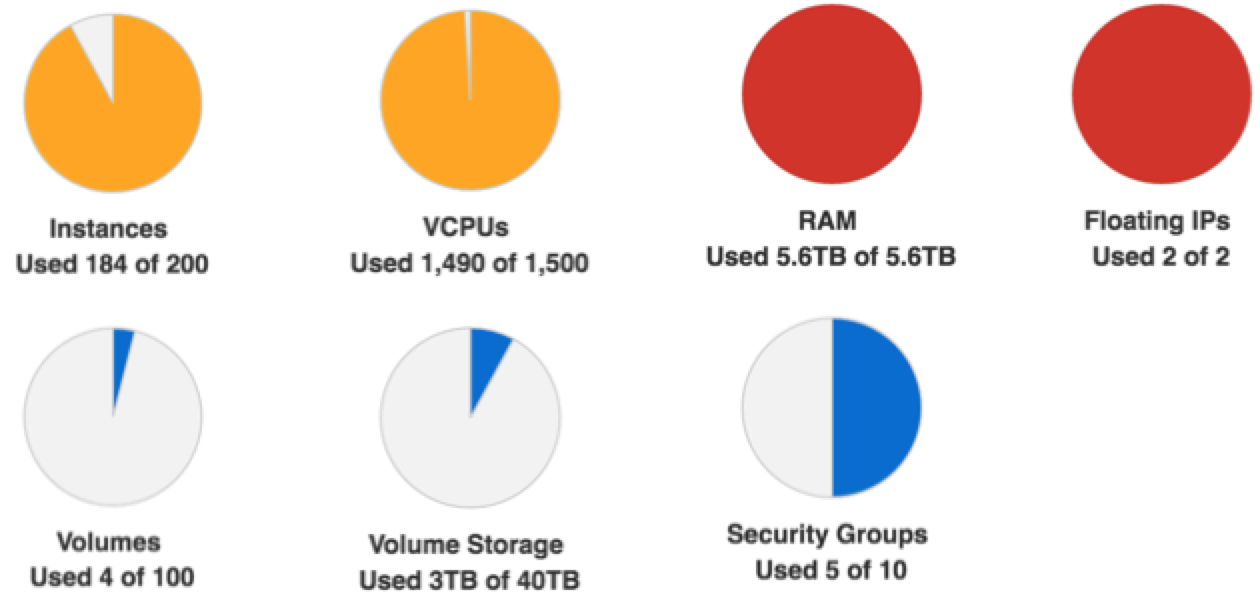
\includegraphics[width=\textwidth]{embassy_dashboard}
\centering
\caption {Embassy Cloud Dashboard}
\label{fig:embassy_dashboard}
\end{figure}

\subsubsection{Access to PCAWG Data}
\label{sec:pcawg_data_access}

The raw data for PCAWG is hosted in a distributed manner in GNOS repositories. A data synchronization mechanism copies data between repositories when necessary. The EMBL/EBI GNOS repository is one of the most complete sources of PCAWG data, hosting close to 1PB of data for the project. Although typically access to the GNOS repository is only available via a GNOS client the Embassy Cloud IT team has made a special provision for the Germline Working Group to allow access to the underlying data via an NFS share. This allows Butler-based workflows to have more efficient access to the data.

The PCAWG project periodically publishes an official list of all samples that are part of the project. In order to facilitate accurate sample tracking for analysis purposes we have built a Sample Tracking Database on top of PostgreSQL and SQLAlchemy. There are two tables \mintinline{sql}{pcawg_samples} and \mintinline{sql}{sample_locations}. \mintinline{sql}{pcawg_samples} maintains a list of official samples along with their accompanying metadata while \mintinline{sql}{sample_locations} contains a set of file paths that indicate where to find each sample on the Embassy Cloud file server. This table is populated by a script that crawls the directory structure looking for samples that are part of the official list.

\subsubsection{Butler deployment}

Butler has been deployed on the Embassy Cloud since March, 2016 and has been used extensively to carry out analyses for the Germline Working Group.

To deploy Butler on the 1500 core cluster we set up five different profiles of VMs, each playing a number of different roles (Table \ref{tab:embassy_deployment}):

\begin{table}[H] 
\renewcommand{\arraystretch}{2} 
\centering
\begin{tabu} to \linewidth {X[3]X[1,r]X[2,r]X[4]X[4]X[1,r]}
\toprule
Machine & CPU & RAM (GB) & Disk (GB) & Roles & Count\\
\midrule
salt-master & 4 & 6 & 50 ephemeral\newline 1000 block for metrics storage & salt-master \newline consul-bootstrap\newline monitoring-server & 1\\
tracker & 4 & 4 & 40 ephemeral \newline 1000 block for elasticsearch & tracker \newline consul-server \newline elasticsearch & 1\\
job-queue & 4 & 4 & 40 ephemeral & job-queue \newline consul-client & 1\\
db-server & 8 & 16 & 80 ephemeral \newline1000 block for db & db-server \newline consul-client & 1\\
worker & 8 & 32 & 100 ephemeral & worker \newline germline \newline consul-client & 175\\
\bottomrule
\end{tabu}
\caption{Butler deployment on Embassy Cloud}
\label{tab:embassy_deployment}
\end{table} 

Each profile is defined separately via Terraform and uses Saltstack roles for configuration. The user can check out the Butler github repository to their local machine and once they install Terraform locally, and provided that they are able to connect to the EBI Secure Gateway (Figure \ref{fig:embassy_architecture}) they can fully commandeer the provisioning process from the local machine via Terraform.

Figure \ref{fig:embassy_butler_deployment_architecture} provides a diagrammatic view of the deployment of various Butler components on the Embassy Cloud.

\begin{figure}[H]
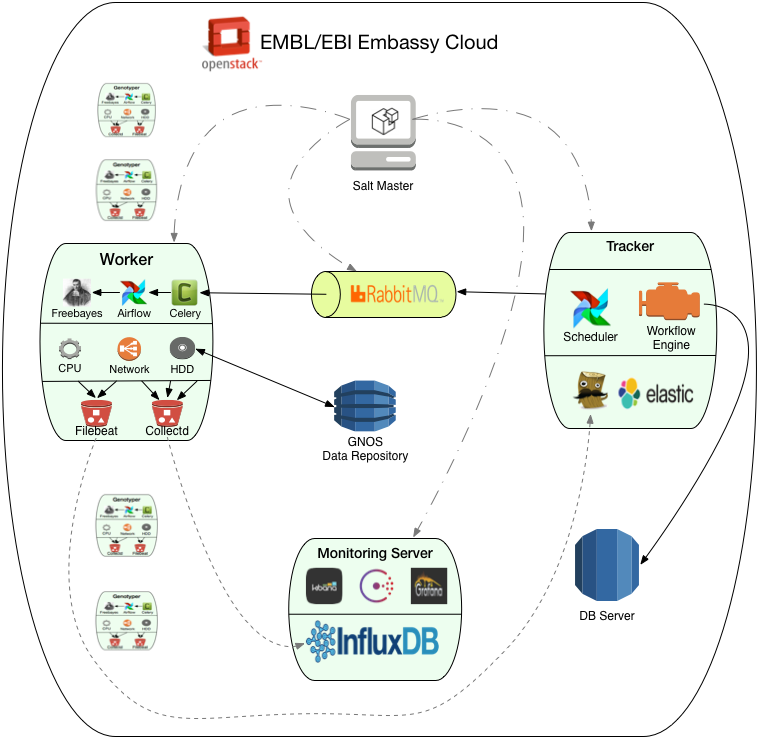
\includegraphics[width=\textwidth]{embassy_butler_deployment_architecture}
\centering
\caption {Butler Deployment Architecture}
\label{fig:embassy_butler_deployment_architecture}
\end{figure}

The cluster is bootstrapped via the salt-master VM. This VM is started first whenever the cluster needs to be recreated from scratch. The salt-master is started with a minimal OS image for speed and all of the other configurations are delivered via Saltstack itself. The IP of the salt-master machine is retained so that it can be passed on to the other VMs upon creation so that they know how to connect to the master when they boot up. The salt-master VM plays two other roles (Table \ref{tab:embassy_deployment}) in this deployment in order to maximize resource utilization (since Saltstack is a light resource consumer) - consul-bootstrap, and monitoring-server. The consul-bootstrap role conveys the responsibility for starting up the Consul Service Discovery mechanism to the salt-master. When set up in bootstrap mode, consul waits for one more consul server to join the cluster, before quorum is reached and the cluster becomes fully operational. The monitoring-server role is responsible for installing and configuring InfluxDB and other monitoring components  as well as registering them with Consul so that metrics can start being recorded. We also attach a 1TB block storage volume for the metrics database so that it can survive cluster crashes and tear-downs. If the monitoring server needs to be recreated, the block storage volume simply needs to be reattached to the new Monitoring Server VM.

The tracker VM is responsible for running various Airflow components such as the - Scheduler, Webserver, and Flower (Section \ref{sec:design_workflow_system}). Additionally we deploy the Butler tracker module (Section \ref{sec:analysis_tracker})to this VM, thus the tracker VM acts as the main control point of the system from which analyses are launched and monitored. This VM additionally has the elasticsearch role which designates it as the location of the Logstash and Elasticsearch components (Section \ref{sec:design_log_collection}). To persist the search index we attach an additional 1TB block storage volume. The consul-server role allows the cluster, once the tracker VM is brought up, to reach quorum necessary for full Consul functionality. 

The job-queue VM is responsible for hosting the RabbitMQ server which holds all of the in-flight workflow tasks. Because the resources of the job-queue are heavily taxed by communication with all of the worker VMs in the cluster we do not assign any additional roles to this host.

The db-server is responsible for hosting most of the databases used by Butler. This VM runs an instance of PostgreSQL Server and hosts the Run Tracking DB, Airflow DB, and Sample Tracking DB. The 1TB block storage volume serves as the backing storage mechanism. 

The worker VMs are the workhorses of the Butler cluster. In its current deployment (October 2016) there are 175 8-core worker machines that are dedicated to running Butler workflows. The worker role ensures that Airflow client modules are installed and loaded on each worker. The germline role additionally loads the workflows and analyses that are relevant to the PCAWG Germline Working Group. 


\section{PCAWG Germline Analyses}

The PCAWG project is divided into a set of working groups. Each group has a different set of research interests and technical activities that it is contributing to the overall project effort.  The goal of the Germline Working Group, also known as PCAWG-8, is to study the distribution of germline (mutations that are inherited from one's parents) polymorphisms within the PCAWG cohort of 2834 cancer patients and gain a better understanding of how these germline polymorphisms affect various aspects of the patients' disease, for instance whether they affect disease progression, likelihood of survival, or any number of molecular-level traits such as DNA repair, propensity towards certain types of mutations, or gene dysregulation.

To enable these analyses the goal of the Germline Working Group is to produce a full set of high quality genotyped germline variants. Doing so requires carrying out a significant number of computational steps that use the entire 725 TB raw data set. These steps are as follows:

\begin{description}
\item [Variant Discovery] - Use a set of algorithms that look at each location in the genome and try to determine where the genome differs from the known reference sequence.
\item [Variant Genotyping] - Using a set of variant sites produced by Variant Discovery and determine an accurate genotype at the variant position for all donors in the cohort.
\item [Variant Filtration] - Filter out false positive calls introduced by the previous steps.
\item [Genotype Phasing] - Use an algorithm to determine which chromosome (of the pair) each variant belongs to.
\item [Data Submission] - Prepare metadata and submit the resulting call-set to a centralized data repository.
\end{description}

\subsection{Variant Discovery}
\label{sec:variant_discovery}

There exist multiple algorithms for variant discovery and each algorithm has a unique set of features. As a result, they typically produce call-sets that only overlap on a subset of the values\autocite{li2014towards}. In order to improve the sensitivity of the call-set the Germline Working Group is producing three independent discovery call sets via three different algorithms - Freebayes\autocite{garrison2012haplotype}, GATK HaplotypeCaller\autocite{depristo2011framework}, and RTG\autocite{cleary2014joint}. These call-sets are then merged via a two-out-of-three criterion i.e. a variant is retained if it is called by at least 2 of the three pipelines. This approach produces a more sensitive call-set than via any of the tools individually.

The GATK HaplotypeCaller data set has been produced by the Broad Institute, the RTG set has been produced by Stanford University, and the Freebayes data set has been produced using a Butler workflow on the EBI Embassy Cloud.

\subsubsection{The freebayes Butler workflow}
The freebayes workflow parallelizes its work by splitting each sample by chromosome to reduce the amount of time it takes to process a single sample. Although the chromosomes have vastly different sizes (see Table \ref{tab:chromosome_sizes}), and thus individual jobs have different runtimes, when many samples are processed, there is little practical impact on when the entire batch of samples is completed.

\begin{table}[H]
\label{tab:chromosome_sizes}
\renewcommand{\arraystretch}{1.2} 
\centering
\begin{tabular}{@{}lll@{}}
\toprule
Chromosome & Size(base pairs)\\
\midrule
1 & 249,250,621\\
2 & 243,199,373\\
3 & 198,022,430\\
4 & 191,154,276\\
5 & 180,915,260\\
6 & 171,115,067\\
7 & 159,138,663\\
8 & 146,364,022\\
9 & 141,213,431\\
10 & 135,534,747\\
11 & 135,006,516\\
12 & 133,851,895\\
13 & 115,169,878\\
14 & 107,349,540\\
15 & 102,531,392\\
16 & 90,354,753\\
17 & 81,195,210\\
18 & 78,077,248\\
19 & 59,128,983\\
20 & 63,025,520\\
21 & 48,129,895\\
22 & 51,304,566\\
X & 155,270,560\\
Y & 59,373,566\\
\bottomrule
\end{tabular}
\caption{Human chromosome size distribution}
\end{table}

Overall, most Butler workflows that carry out an analysis follow a similar structure - an Analysis Run is started, access to the sample is validated, the analysis steps are carried out (possibly with branching), and the Analysis Run is completed (see Figure \ref{fig:butler_freebayes_workflow}).

\begin{figure}[H]
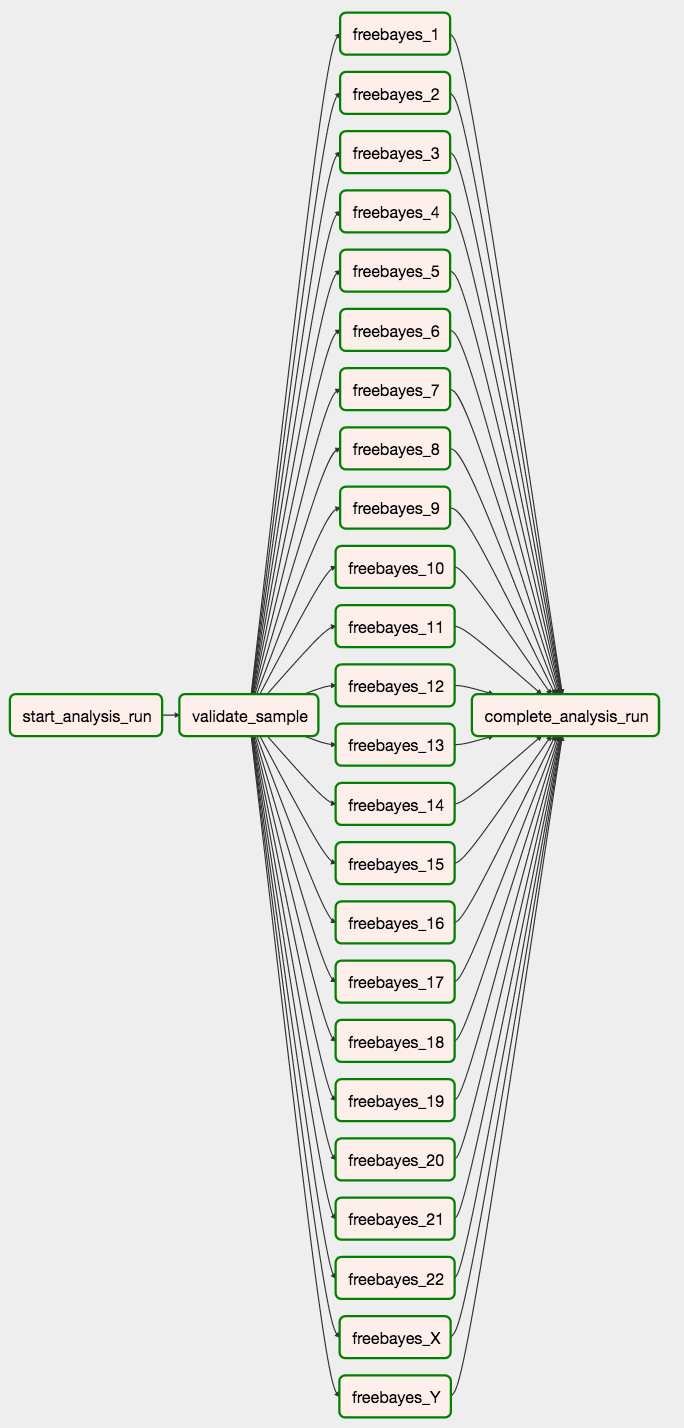
\includegraphics[scale=0.7]{butler_freebayes_workflow}
\centering
\caption {Structure of the Butler freebayes workflow}
\label{fig:butler_freebayes_workflow}
\end{figure}

Because of the largely common structure between workflows a large degree of code reuse is possible, thus most of the methods reside in the workflow\_common submodule of the tracker module (see Section \ref{sec:analysis_tracker}) and are invoked for each workflow.

A full listing of the source code for the freebayes workflow is provided in Listing \ref{lst:freebayes_workflow} and is discussed next. 




Lines 81-127 of the source code define the workflow structure, first by declaring an instance of type \mintinline{python}{DAG}, and then by defining a sequence of workflow tasks. In this case each task is a Python callable. The loop on line 117 defines one workflow task for each chromosome in the predefined list. The order of task execution is defined by calling a task's \mintinline{python}{set_upstream()} method, such as on lines 109 and 127 of the listing. Default parallelism behaviour is specified on line 92 where the maximum number of active workflow runs is defined to be 2000, and the maximum number of active workflow tasks is defined to be 10,000. If more workflows than the maximum get scheduled, they will be queued until some workflow instances complete.

The bulk of the body of the workflow definition (lines 14-78) is dedicated to the implementation of a single function - \mintinline{python}{run_freebayes(**kwargs)} which manages the invocation of the freebayes tool on a single chromosome of a sample. Line 16 gets the effective configuration dictionary (see Section \ref{sec:workflow_configuration_design}) which contains the merged configuration parameters from Workflow (Listing \ref{lst:freebayes_workflow_config}), Analysis (Listing \ref{lst:freebayes_discovery_config}), and Analysis Run (Listing \ref{lst:freebayes_discovery_run_config}) levels. 


\captionof{listing}{Workflow-level configuration for freebayes workflow.\label{lst:freebayes_workflow_config}}
\begin{minted}
[
breaklines=true,
linenos,
fontsize=\footnotesize,
frame=lines,
framesep=2mm,
baselinestretch=1.2
]
{json}
{
	"contig_names": ["1", "2", "3", "4", "5", "6", "7", "8", "9", "10",
                "11", "12", "13", "14", "15", "16", "17", "18", "19", 
                "20", "21", "22", "X", "Y"],
	"reference_location": "/reference/genome.fa",
	"bgzip": {
		"path": "/usr/local/bin/bgzip",
		"flags": ""
	},
	"tabix": {
		"path": "/usr/local/bin/tabix",
		"flags": "-f -p vcf"
	},
	"rsync": {
		"flags": "-a -v --remove-source-files"
	},
	"freebayes": {
		"path": "/bin/freebayes"
	}
}
\end{minted}

The workflow-level configurations contain values that should generally be applicable to any invocation of the workflow. In exceptional cases these can be overridden at Analysis and 
Analysis Run levels. For the freebayes workflow these settings include a list of chromosomes to call, the path to the human reference genome, and paths to various tools used within the workflow

\captionof{listing}{Analysis-level configuration for freebayes variant discovery analysis.\label{lst:freebayes_discovery_config}}
\begin{minted}
[
breaklines=true,
linenos,
fontsize=\footnotesize,
frame=lines,
framesep=2mm,
baselinestretch=1.2
]
{json}
{
	"results_base_path": "/shared/data/results/discovery/",
	"results_local_path": "/tmp/discovery/",
	"freebayes": {
		"mode": "discovery",
		"flags": "--min-repeat-entropy 1 --report-genotype-likelihood-max"
	}
}
\end{minted}

Since our analysis focuses on variant discovery, the Analysis-level JSON configuration file contains freebayes flags to set up discovery mode, as well as setting up a location for where to store the analysis results and which directory to use as local scratch space.
 
\captionof{listing}{AnalysisRun-level configuration for a single sample in freebayes variant discovery analysis. \label{lst:freebayes_discovery_run_config}}
\begin{minted}
[
breaklines=true,
linenos,
fontsize=\footnotesize,
frame=lines,
framesep=2mm,
baselinestretch=1.2
]
{json}
{
	"sample": {
		"sample_location": "/gnosdata/tcga/PCAWG.67455c36-aa47-4cc4-8b6d-9a9012b616ed.bam",
		"donor_index": 0,
		"sample_id": "f22a72c5-73c8-478d-b03e-04599b9d5321"
	}
}
\end{minted}

Listing \ref{lst:freebayes_discovery_run_config} provides an example of what an AnaysisRun-level configuration looks like. This configuration is concerned with supplying sample level configuration values, such as the sample\_id and sample\_location.

After all of the necessary parameters are extracted from the configuration and command invocation is set up lines 71-75 of Listing \ref{lst:freebayes_workflow} actually invoke a series of commands that perform the bulk of the analysis - calling \mintinline{shell}{freebayes} to generate the discovery call-set, followed by converting the call-set into a binary compressed format (with \mintinline{shell}{bgzip}), followed by generating an index file for record-based random access into the binary file (with \mintinline{shell}{tabix}), and followed by an \mintinline{shell}{rsync} to the shared results storage indicated in the configuration.

The workflow is distributed to all worker nodes in the cluster via a Saltstack state as shown in Listing \ref{lst:workflow_deployment}.



\subsubsection{AnalysisRun configurations for freebayes workflow}

While each workflow only has one workflow-level configuration and possibly a few dozen analysis-level configurations, there needs to be one analysis run-level configuration generated for each sample under analysis, thus resulting in thousands of these configurations being generated for each analysis. The most effective method for accomplishing this is via a script. We utilize two databases - the Run Tracking Database (Section \ref{sec:analysis_tracker}), and the Sample Tracking Database (Section \ref{sec:pcawg_data_access}) in order to generate a list of samples for which there are no Analysis Runs present for a given Analysis yet. To generate our result-set we utilize the SQLAlchemy Object-Relational Mapping framework (see \ref{sec:available_samples}).

\captionof{listing}{SQLAlchemy query to generate available samples.\label{lst:available_samples}}
\begin{minted}
[
breaklines=true,
fontsize=\footnotesize,
linenos,
frame=lines,
framesep=2mm,
baselinestretch=1.2
]
{python}
current_runs = run_session.query(Configuration.config[("sample"," sample_id")].astext).\
        join(AnalysisRun, AnalysisRun.config_id == Configuration.config_id).\
        join(Analysis, Analysis.analysis_id == AnalysisRun.analysis_id).\
        filter(and_(Analysis.analysis_id == analysis_id, AnalysisRun.run_status != tracker.model.analysis_run.RUN_STATUS_ERROR)).all()
        
available_samples = sample_session.query(PCAWGSample.index.label("index"), sample_id.label("sample_id"), sample_location.label("sample_location")).\
        join(SampleLocation, PCAWGSample.index == SampleLocation.donor_index).\
        filter(and_(sample_location != None, sample_id.notin_(current_runs))).\
        limit(num_runs).all()
\end{minted}

The final script is wrapped in a Command Line Interface to improve the user experience. It supports the following parameters:

\begin{description}
\item [analysis\_id] - The id of the Analysis for which to generate Analysis Run configs.
\item [num\_runs] - The number of runs to generate. The actual number of runs will be \mintinline{shell }{min(num_runs, available_runs)}
\item [tissue\_type] - Whether to generate the Analysis Runs for tumor or normal tissue samples.
\item [config\_location] - File path where to store the resulting Analysis Run configs.
\end{description}

Thus, a full invocation would look like:

\begin{minted}
[breaklines=true]
{shell}
python prepare_freebayes_genotyping_config.py create-configs -a 3 -n 150 -t normal -c /config_file_location/
\end{minted}

This would generate at most 150 JSON files with configurations for Analysis ID 3 and normal tissue samples, storing them in /config\_file\_location/ which could be used to start workflow instances for this analysis.


\subsection{Variant Genotyping}

Genotyping refers to accurately determining for each sample and at each variant position what are the two nucleotide bases (one for each sister chromosome) at that position\autocite{wang1998large}. This analysis involves looking at the DNA reads that overlap each position and evaluating a model for the likelihood of each possible genotype given the data observed in the reads. The genotype with the highest likelihood given the data is selected\autocite{nielsen2011genotype}. To accomplish this task we use a Butler workflow that utilizes freebayes as the computational algorithm underneath the covers. Because the freebayes workflow from Section \ref{sec:variant_discovery} has been built in a generic fashion the only changes that are necessary between discovery and genotyping analyses lie within the analysis configuration.

We see in Listing \ref{lst:genotyping_analysis} that we need to provide a list of variant locations that need to be genotyped, split by chromosome, and stored in VCF format\autocite{danecek2011variant}. Additionally, we provide a set of flags to freebayes that indicate that the tool should be used in genotyping mode.

\subsection{Variant Filtration}

Although utilizing multiple variant callers for variant discovery improves the overall sensitivity it also increases the number of false positives in the call-set. In order to remove the false positive calls the Germline Working Group has undertaken a number of filtration steps. Some of these steps involve machine learning methods that are carried out outside the scope of Butler, but some are based on a set of well-known filtering criteria. These are implemented as a separate Butler workflow.

\begin{figure}[H]
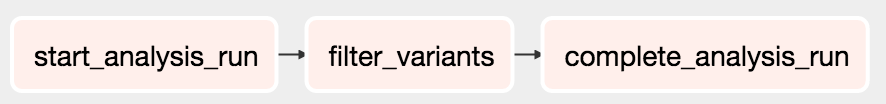
\includegraphics[scale=0.7]{butler_filter_variants_workflow}
\centering
\caption {Structure of the Butler Variant Filtration workflow}
\label{fig:butler_filter_variants_workflow}
\end{figure}

The Filter Variants workflow has a rather simple structure. Bookended by the standard run-start and run-completion tasks is the actual filtration task. This task is implemented as an Airflow PythonOperator and invokes two commands - vcftools\autocite{danecek2011variant} and vt\autocite{tan2015unified}. vcftools is used for actual variant filtering, while vt is used for variant normalization.

\captionof{listing}{Butler Analysis configuration for VCF filtering.\label{lst:filtering_analysis}}
\begin{minted}
[
breaklines=true,
breakanywhere=true,
fontsize=\footnotesize,
linenos,
frame=lines,
framesep=2mm,
baselinestretch=1.2
]
{json}
{
	"results_base_path": "/shared/data/results/discovery_filtered/",
	"results_local_path": "/tmp/discovery_filtered/",
	"vcffilter": {
		"flags": "QUAL > 20 & DP > 3 & QUAL / AO > 2 & SAF > 1 & SAR > 1 & RPR > 1 & RPL > 1"
	},
	"vt": {
		"command": "normalize"
	}
}
\end{minted}

Listing \ref{lst:filtering_analysis} demonstrates the usage of vcftools' flags to achieve variant filtering for PCAWG. 

\subsection {Genotype Phasing}

Because each individual inherits one copy of each chromosome (except for sex chromosomes X and Y) from the mother and one from the father, a variant may lie on one chromosome or the other, or both. It is, thus, important to understand which chromosome each variant lies on in order to inform downstream analyses. This methodology is called statistical phasing and will be carried out by a tool called Shapeit\autocite{delaneau2012linear} outside of Butler.

\subsection {Data Submission}

Once a call-set for each sample is produced and vetted it needs to be submitted to a centralized data repository so that it can be shared with other researchers on the project. There are seven such data repositories throughout the world, each running a software tool called GNOS\autocite{wilks2014cancer} from Annai Systems. A submission to GNOS consists of the call-set data accompanied by an XML-formatted metadata file, that describes the submission. GNOS then uses a proprietary torrent-like protocol for secure file uploads. A Butler workflow implements automated sample submissions to GNOS.

\begin{figure}[H]
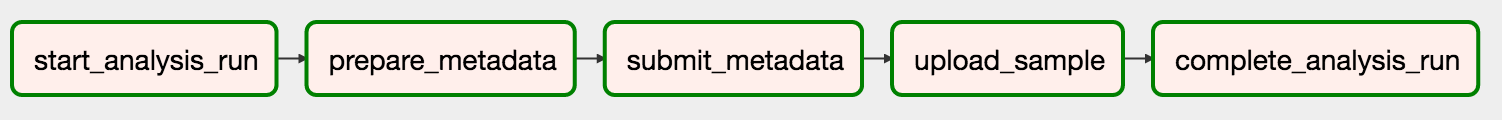
\includegraphics[width=\textwidth]{butler_gtupload_workflow}
\centering
\caption {Structure of the Butler Data Submission workflow}
\label{fig:butler_gtupload_workflow}
\end{figure}

The Data Submission workflow (Figure \ref{fig:butler_gtupload_workflow}) follows a linear sequence of events implemented as Airflow PythonOperators. The data submission is a three step process where the first action is to prepare a sample's accompanying metadata submission, the second is to submit this metadata to a GNOS repository of choice, which generates a manifest in return, and the third step is to upload the actual data to the same repository using the manifest. See Listing \ref{lst:gtupload_workflow}

In order to be able to successfully submit a sample, the sample, along with its accompanying metadata must be placed in a separate directory whose name is a Universally Unique Identifier (UUID) - this UUID will become an identifier for the submission on the GNOS server. Furthermore, the metadata file - an XML document, must be populated with descriptions of the analysis steps taken to produce the sample. We generate this file in Butler's workflow with the aid of an XML template (see Listing \ref{lst:gtupload_analysis} template declaration) and using Python's \mintinline{python}{etree} module.


Once the submission is ready, the actual process of submission is carried out using the \mintinline{shell}{cgsubmit} tool by Annai Systems. It is important which GNOS repository a sample ends up in as not all repositories have permissions to host all samples. The \mintinline{shell}{destination_repo_mapping} dictionary in Listing \ref{lst:gtupload_analysis} maintains a mapping between a sample's project and a corresponding GNOS repository name. Listing \ref{lst:gtupload_workflow} provides a further mapping between repository names and repository URLs thus allowing \mintinline{shell}{cgsubmit} to submit each sample to its corresponding GNOS repository. The output of the metadata\_submit task is a \mintinline{shell}{manifest.xml} file which is placed in the sample's directory and contains all of the necessary information to enable the upload of the actual data.

The upload\_data task is responsible for moving the actual data into a designated GNOS repository. This is accomplished using a tool called \mintinline{shell}{gtupload} which implements a torrent-like data upload protocol. 

\subsection {Structural Variant Calling}

While the previously described methods are geared towards the detection and genotyping of Single Nucleotide Polymorphisms (SNPs), there are other classes of germline variants within a person's genome. Structural Variants form a broad class of larger polymorphisms which are typically 50 basepairs or larger in size\autocite{sudmant2015integrated}. There are various types of structural variants, including:

\begin{itemize}
\item Deletions
\item Inversions
\item Duplications
\item Translocations
\end{itemize}

The Germline Working Group is using a tool called Delly\autocite{rausch2012delly} to accurately detect and genotype these variants. To enable Delly analyses on the EBI Embassy Cloud we have built a Delly workflow in Butler (Figure \ref{fig:butler_delly_workflow}).

\begin{figure}[H]
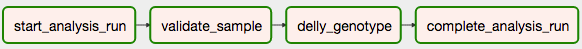
\includegraphics[width=\textwidth]{butler_delly_workflow}
\centering
\caption {Structure of the Butler Delly workflow}
\label{fig:butler_delly_workflow}
\end{figure}

This workflow has a familiar linear structure with the bulk of the work being done inside the delly\_genotype task. Because Delly knows how to work with and output compressed VCF files there is no need to compress and generate indexes like with freebayes. This makes the task code simpler (Listing \ref{lst:run_delly}).


After extracting the necessary configuration parameters and setting up the delly execution command, once delly execution finishes, the resulting call-set is copied over to its final location. Control over program behaviour is mostly exercised at the analysis level, where program flags are typically indicated (Listing \ref{lst:delly_analysis})

\section{Experimental Runs}

Between January and October 2016 Butler has been used extensively to facilitate a number of large scale cancer genomics analyses on behalf of the Germline Working Group of the Pan Cancer Analysis of Whole Genomes Project. The input to these analyses has been a 725 TB data-set of 2834 cancer patients' sequenced DNA samples, and the outputs have been a number of call-sets identifying and genotyping various classes of germline variants in the form of VCF files. All of the computations have been performed on the EMBL/EBI Embassy Cloud - a 1500 core, 6TB of RAM, 1PB of storage, academic cloud running Openstack.

In this section we describe the technical details and characteristics of these experimental runs to establish a measure of Butler's effectiveness in real-life scenarios.

\subsection{Freebayes Common Variant Genotyping}

The Common Variant Genotyping analysis refers to the genotyping within the PCAWG cohort the genomic variants that occur with at least 1\% Minor Allele Frequency (MAF) within the 1000 Genomes Project's\autocite{10002012integrated} cohort. This site list consists of ~12 million variants that need to be genotyped for each patient - thus requiring genotyping at 34 billion sites.

To accomplish this task we utilize the Butler freebayes workflow in genotyping mode, supplying the following configurations:

\captionof{listing}{Butler Freebayes Workflow analysis configuration for common variants genotyping.\label{lst:analysis_1_percent_maf}}
\begin{minted}
[
breaklines=true,
breakanywhere=true,
fontsize=\footnotesize,
linenos,
frame=lines,
framesep=2mm,
baselinestretch=1.2
]
{json}
{
	"variants_location": {
		"1": "/1000GP_maf_0.01/ALL.chr1.vcf.gz",
	        "2": "/1000GP_maf_0.01/ALL.chr2.vcf.gz",
	        "3": "/1000GP_maf_0.01/ALL.chr3.vcf.gz",
	        "4": "/1000GP_maf_0.01/ALL.chr4.vcf.gz",
	        "5": "/1000GP_maf_0.01/ALL.chr5.vcf.gz",
	        "6": "/1000GP_maf_0.01/ALL.chr6.vcf.gz",
	        "7": "/1000GP_maf_0.01/ALL.chr7.vcf.gz",
	        "8": "/1000GP_maf_0.01/ALL.chr8.vcf.gz",
	        "9": "/1000GP_maf_0.01/ALL.chr9.vcf.gz",
	        "10": "/1000GP_maf_0.01/ALL.chr10.vcf.gz",
	        "11": "/1000GP_maf_0.01/ALL.chr11.vcf.gz",
	        "12": "/1000GP_maf_0.01/ALL.chr12.vcf.gz",
	        "13": "/1000GP_maf_0.01/ALL.chr13.vcf.gz",
	        "14": "/1000GP_maf_0.01/ALL.chr14.vcf.gz",
	        "15": "/1000GP_maf_0.01/ALL.chr15.vcf.gz",
	        "16": "/1000GP_maf_0.01/ALL.chr16.vcf.gz",
	        "17": "/1000GP_maf_0.01/ALL.chr17.vcf.gz",
	        "18": "/1000GP_maf_0.01/ALL.chr18.vcf.gz",
	        "19": "/1000GP_maf_0.01/ALL.chr19.vcf.gz",
	        "20": "/1000GP_maf_0.01/ALL.chr20.vcf.gz",
	        "21": "/1000GP_maf_0.01/ALL.chr21.vcf.gz",
	        "22": "/1000GP_maf_0.01/ALL.chr22.vcf.gz"
	},
	"results_base_path": "/shared/data/results/regenotype_1_percent_maf/",
	"results_local_path": "/tmp/regenotype_1_percent_maf/",
	"freebayes": {
		"mode": "regenotyping",
		"flags": "-l"
	}
}
\end{minted}

Figure \ref{fig:freebayes_1_percent_maf_genotyping} shows a distribution of job runtimes (in minutes) separated by chromosome. The mean runtime is highly correlated with chromosome length (and consequently number of variants), with a Pearson correlation of 0.92.

\begin{figure}[H]
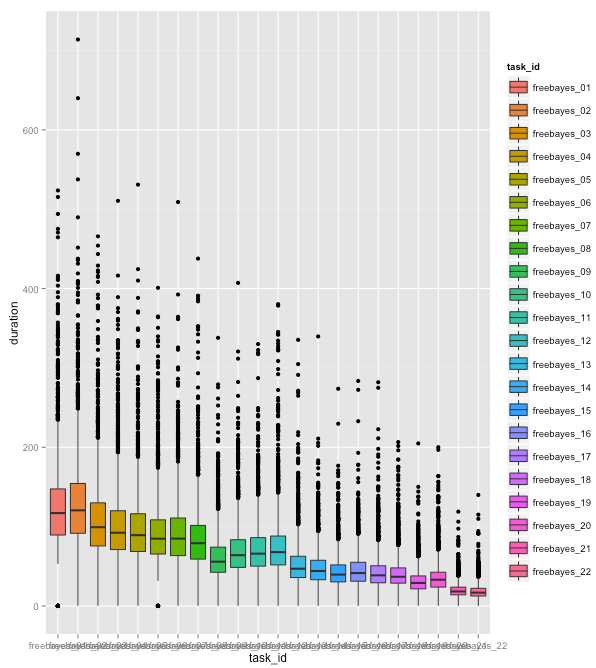
\includegraphics[scale=0.6]{freebayes_1_percent_maf_genotyping}
\centering
\caption {Runtimes of freebayes genotyping on the 1\% MAF site-list.}
\label{fig:freebayes_1_percent_maf_genotyping}
\end{figure}

Overall 130,152 compute hours were used to complete 70,850 workflow tasks for this analysis with an additional 2688 CPU hours used for cluster management overhead. Thus, management overhead accounted for ~2\% of the overall computational resource costs for this analysis. Utilizing 1000 cores this analysis took less than 6 days to complete.

\subsection{Freebayes Variant Discovery}
\subsection{Freebayes Variant Genotyping}

Using the site-list of 60 million variants obtained from the Freebayes Variant Discovery analysis we used the Butler Freebayes Workflow in genotyping mode to calculate genotypes at ~170 billion genomic positions. 76,518 tasks workflow tasks were completed utilizing 302,071 CPU hours over the course of the analysis (~10 days wall time), of which 5,040 CPU hours were cluster management overhead, accounting for 1.6\% of total resource utilization. Figure  \ref{fig:freebayes_discovery_regenotype_task_durations} demonstrates the distribution of task durations by chromosome.

\begin{figure}[H]
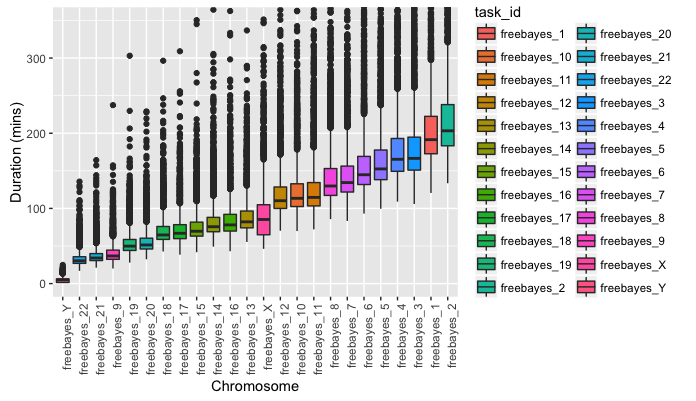
\includegraphics[width=\textwidth]{freebayes_discovery_regenotype_task_durations}
\centering
\caption {Runtimes of freebayes regenotyping on the freebayes discovery call-set.}
\label{fig:freebayes_discovery_regenotype_task_durations}
\end{figure}

Figure \ref{fig:freebayes_discovery_regenotype_task_duration_densities} provides a density-based view of task durations split by chromosome. We observe that durations in each case tend to fall about some mean, dependent on chromosome length (Pearson's r = 0.925), with variance also decreasing with chromosome length (r = 0.94). In each case there is a considerable right tail of duration outcomes, with the maximum duration for each chromosome occurring on average 11.7 standard deviations from the mean.

\begin{figure}[H]
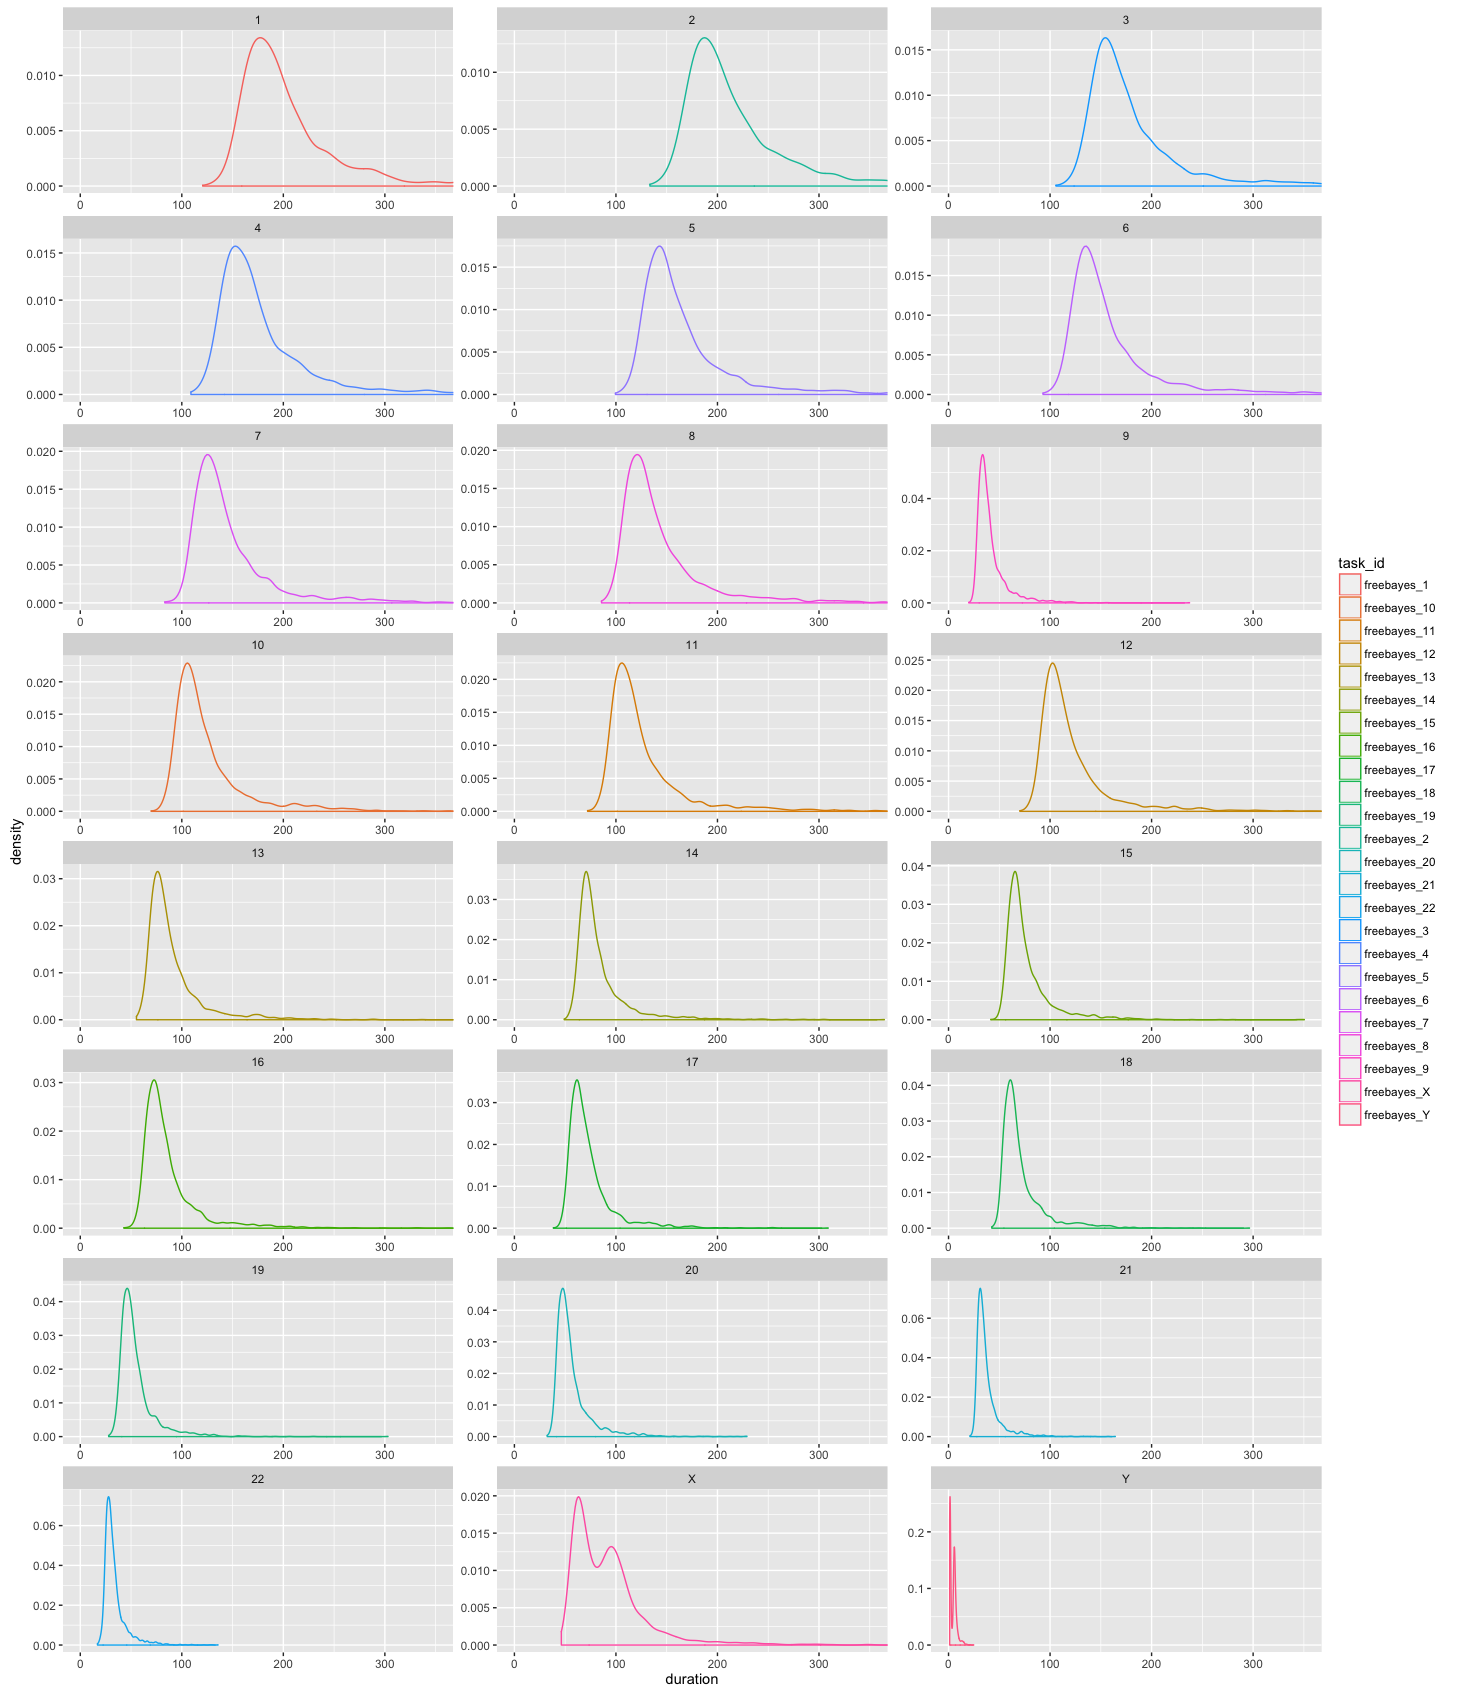
\includegraphics[width=\textwidth]{freebayes_discovery_regenotype_task_duration_densities}
\centering
\caption {Task duration distributions by chromosome.}
\label{fig:freebayes_discovery_regenotype_task_duration_densities}
\end{figure}

Figure \ref{fig:freebayes_discovery_regenotype_cluster_load} shows a view of the cluster load during the analysis execution. Here we see that overall the load has been stable, with a few sporadic spikes (5/25, 5/28, 5/29). On the other hand we see that the load is not uniform across the cluster with some machines not fully utilized. This is clear from the CPU utilization panel, where the majority of the VMs are at 100\% CPU utilization throughout the analysis execution, but several machines appear to be stable at utilization levels between 50\% and 90\%.

\begin{figure}[H]
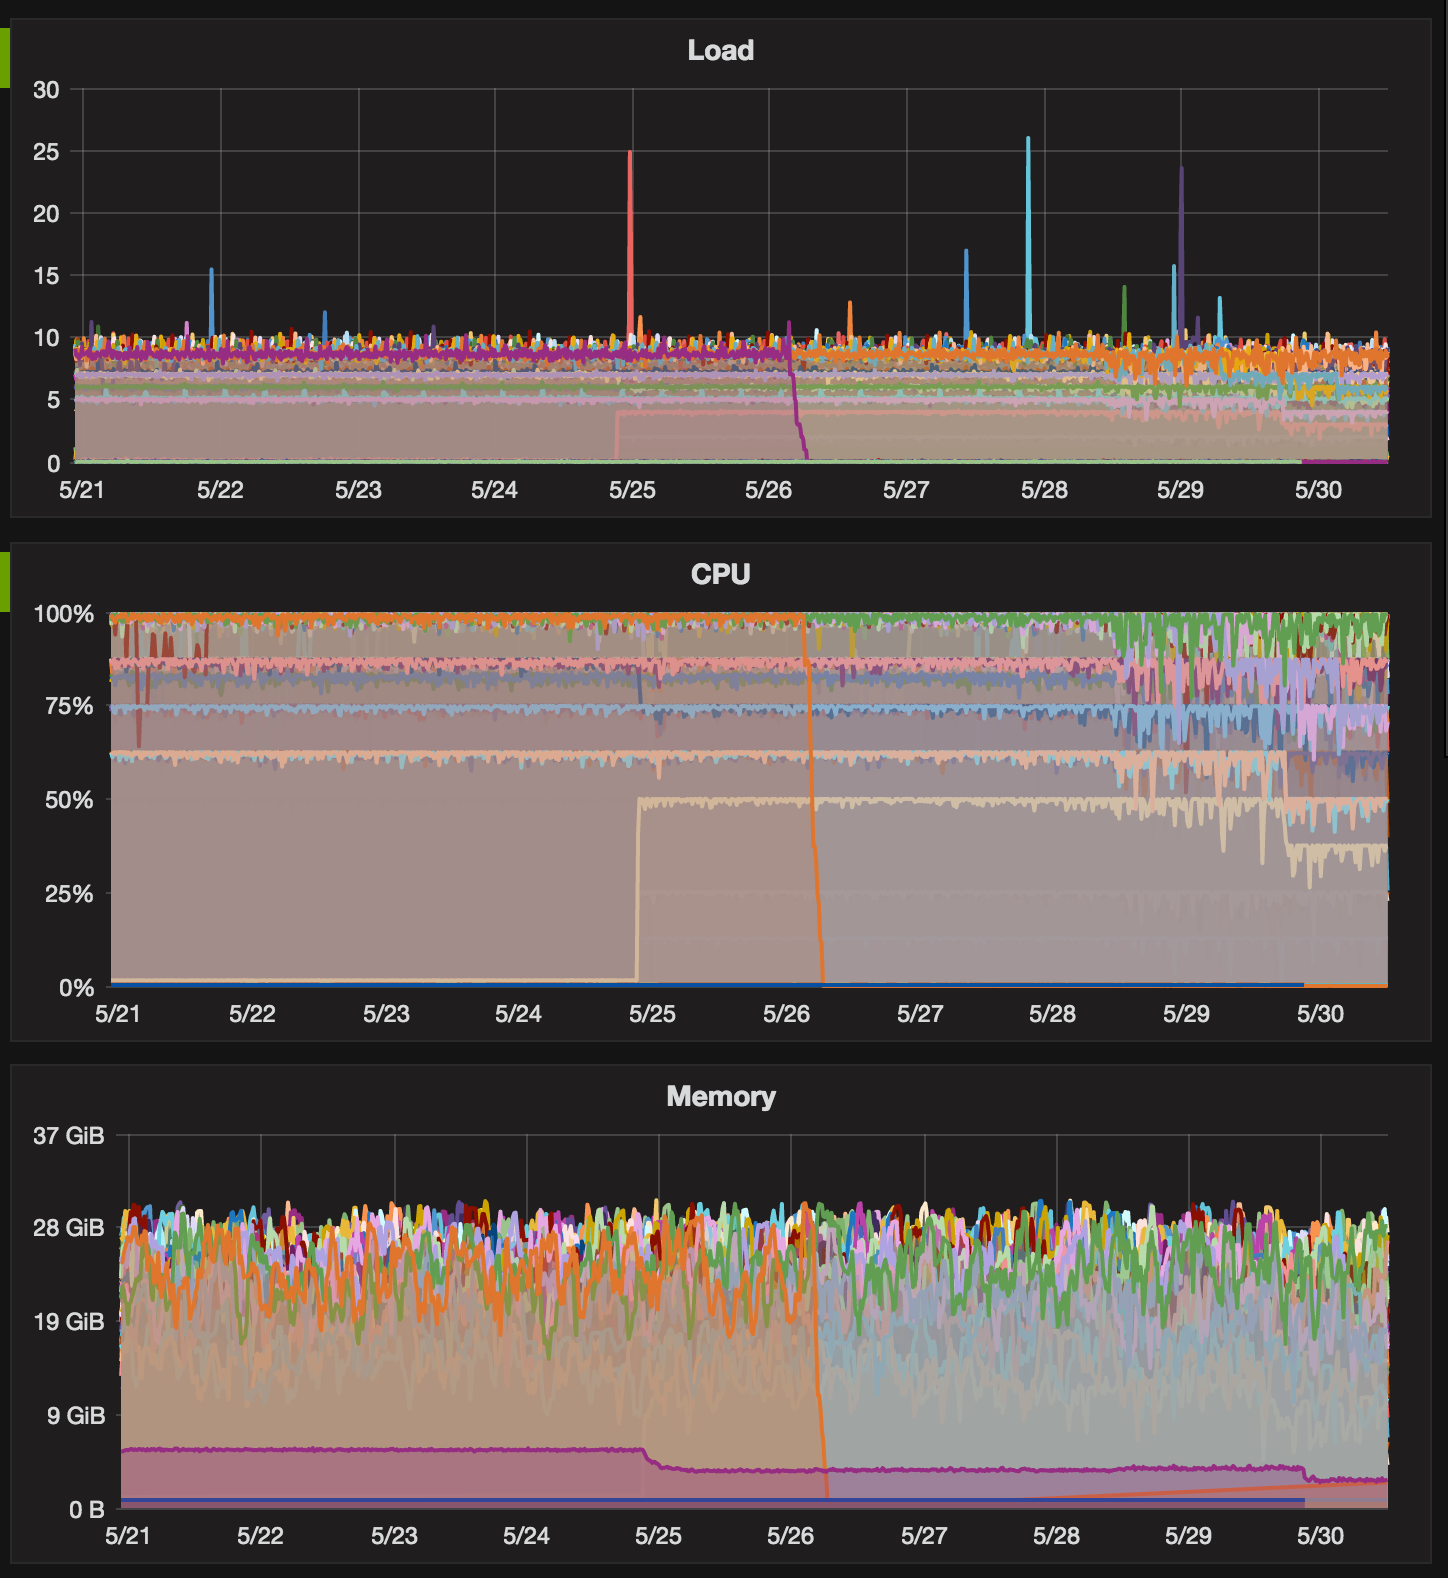
\includegraphics[width=\textwidth]{freebayes_discovery_regenotype_cluster_load}
\centering
\caption {Cluster resource utilization during the regenotyping analysis.}
\label{fig:freebayes_discovery_regenotype_cluster_load}
\end{figure}

\subsection{Delly Full Variant Genotyping}

The analysis of Delly Structural Variant Calling has been split into two parts - genotyping of germline deletions, and genotyping of germline duplications. We consider each in turn.


\subsubsection{Deletions Genotyping}
The deletions analysis used the following analysis configuration:

\captionof{listing}{Butler Delly Workflow analysis configuration for deletions genotyping.\label{lst:delly_analysis_dels}}
\begin{minted}
[
breaklines=true,
breakanywhere=true,
fontsize=\footnotesize,
linenos,
frame=lines,
framesep=2mm,
baselinestretch=1.2
]
{json}
{
	"variants_location": "/shared/data/samples/vcf/delly_deletion_sites/del.sites.bcf",
	"results_base_path": "/shared/data/results/delly_germline_deletions_14_07_2016/",
	"results_local_path": "/tmp/delly_germline_deletions/",
	"variants_type": "DEL"
	
}
\end{minted}
244,889 deletions were evaluated across 5668 samples (tumour and normal) for a total of 1,388,030,852 genomic sites genotyped. Overall wall-time was 13 days, utilizing 265,200 CPU hours with 6240 CPU hours used for cluster management overhead - an overhead of 2.2\%. 

Figure \ref{fig:delly_deletion_durations} shows a histogram of genotyping (sample level) jobs.

\begin{figure}[H]
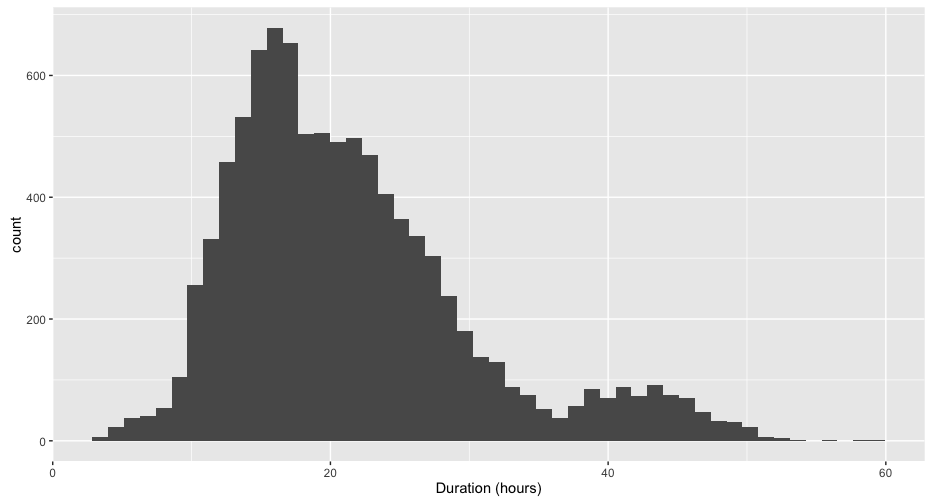
\includegraphics[width=\textwidth]{delly_deletion_durations}
\centering
\caption {Durations of deletion genotyping tasks by sample.}
\label{fig:delly_deletion_durations}
\end{figure}

Table \ref{tab:delly_deletion_summary_stats} shows the summary statistics of job durations.

\begin{table}[H]
\caption {Summary statistics of delly deletion genotyping job durations} \label{tab:delly_deletion_summary_stats}
\centering
\begin{tabular}{lrrrrr}
  \hline
 task\_id & mean & median & sd & min & max \\ 
  \hline
delly\_genotype & 21.48 & 19.70 & 8.89 & 3.35 & 59.30 \\ 
   \hline
\end{tabular}
\end{table}

Figure \ref{fig:delly_deletion_genotyping} shows the overall cluster load during the deletion genotyping analysis. During this analysis there were several periods during which the Workflow Scheduler failed and the job queue ran out of tasks. These periods can be seen as dips on the Load, CPU, and Memory metrics' graphs. 

\begin{figure}[H]
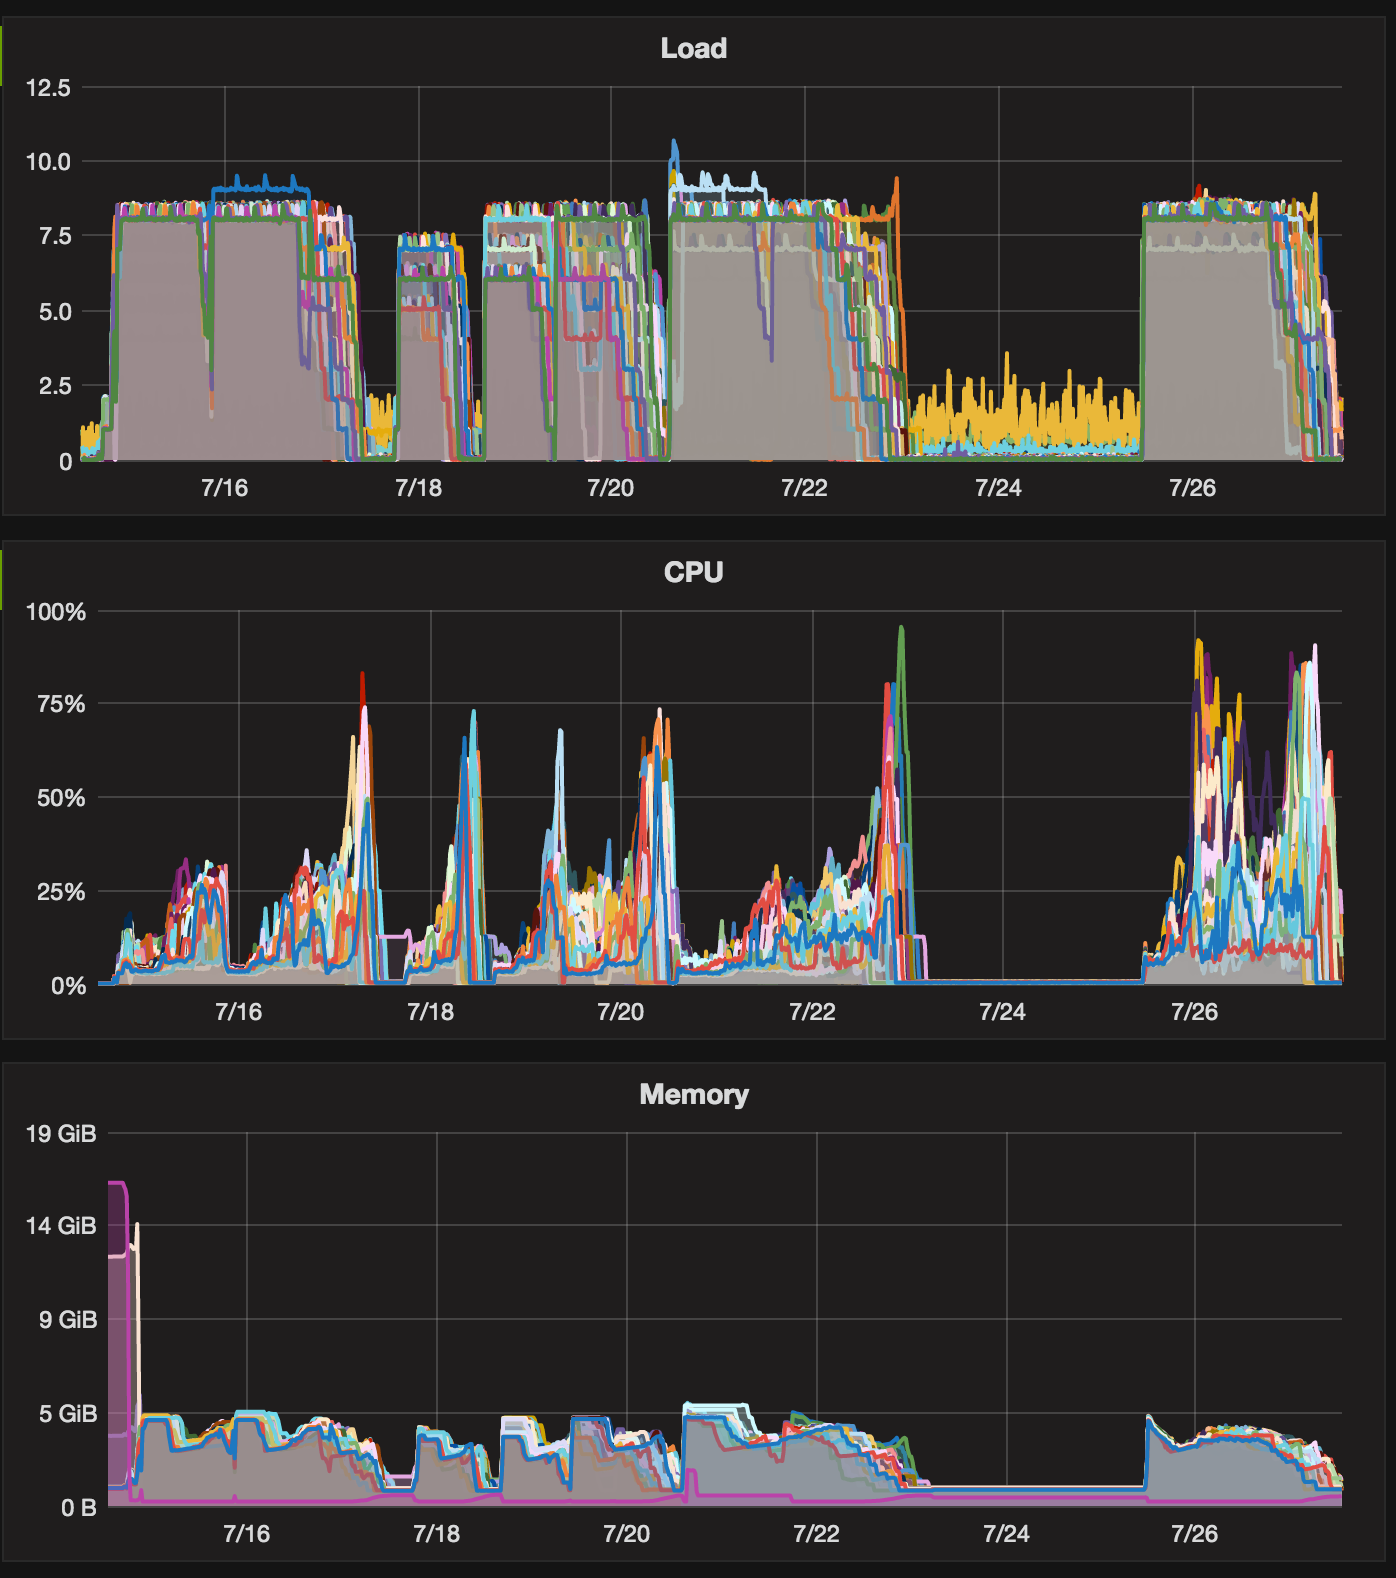
\includegraphics[width=\textwidth]{delly_deletion_regenotyping}
\centering
\caption {Cluster performance during the deletion genotyping analysis.}
\label{fig:delly_deletion_genotyping}
\end{figure}

\subsubsection{Duplications Genotyping}

The duplications analysis used the following configuration:

\captionof{listing}{Butler Delly Workflow analysis configuration for duplications genotyping.\label{lst:analysis_delly_dups}}
\begin{minted}
[
breaklines=true,
breakanywhere=true,
fontsize=\footnotesize,
linenos,
frame=lines,
framesep=2mm,
baselinestretch=1.2
]
{json}
{
	"variants_location": "/shared/data/samples/vcf/delly_deletion_sites/dup.sites.bcf",
	"results_base_path": "/shared/data/results/delly_germline_dups_05_09_2016/",
	"results_local_path": "/tmp/delly_germline_dups/",
	"variants_type": "DUP"
	
}
\end{minted}

Overall 217,433 duplications were genotyped for each sample, across 5668 samples for a total of 1,232,410,244 genomic variants genotyped. The wall-time for this analysis was only 4.5 days, utilizing 151,200 CPU hours during this time, with a management overhead of 2160 hours, for a total overhead of 1.4\%. The comparatively lower cluster management overhead has been accomplished by scaling up the cluster to 1400 cores without the need for more management resources.

Figure \ref{fig:delly_duplication_durations} shows a histogram of genotyping job durations.

\begin{figure}[H]
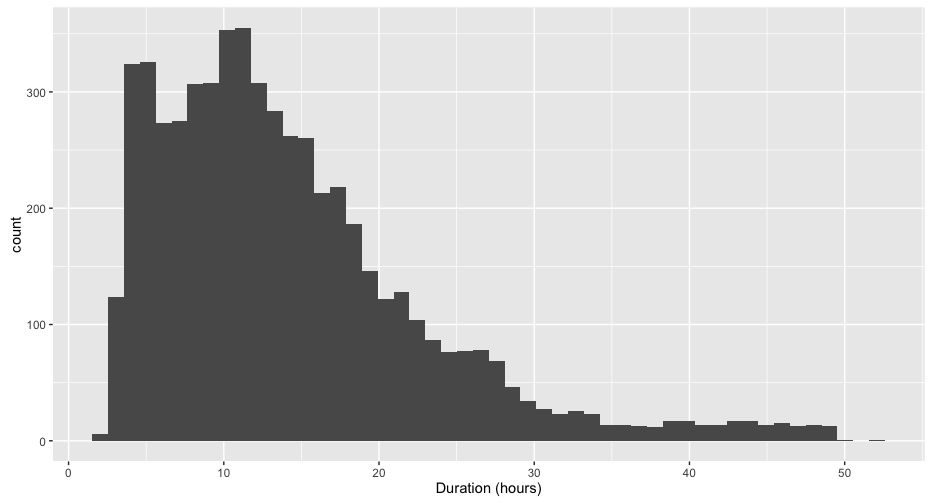
\includegraphics[width=\textwidth]{delly_duplication_durations}
\centering
\caption {Durations of duplication genotyping tasks by sample.}
\label{fig:delly_duplication_durations}
\end{figure}

Table \ref{tab:delly_duplication_summary_stats} provides summary statistics of the same data.

\begin{table}[H]
\caption {Summary statistics of delly duplication genotyping job durations} \label{tab:delly_duplication_summary_stats}
\centering
\begin{tabular}{rlrrrrr}
  \hline
 & task\_id & mean & median & sd & min & max \\ 
  \hline
1 & delly\_genotype & 14.27 & 12.32 & 8.80 & 2.15 & 52.19 \\ 
   \hline
\end{tabular}
\end{table}

Figure \ref{fig:delly_duplication_regenotyping} shows a measurement of cluster performance during the duplication genotyping analysis. This analysis appears to have run very smoothly, with two tranches of data - the normal genomes, and the tumour genomes closely following each other and exhibiting stable Load and Memory performance, and a CPU load profile that is, although spiky, is normal for Delly execution.

\begin{figure}[H]
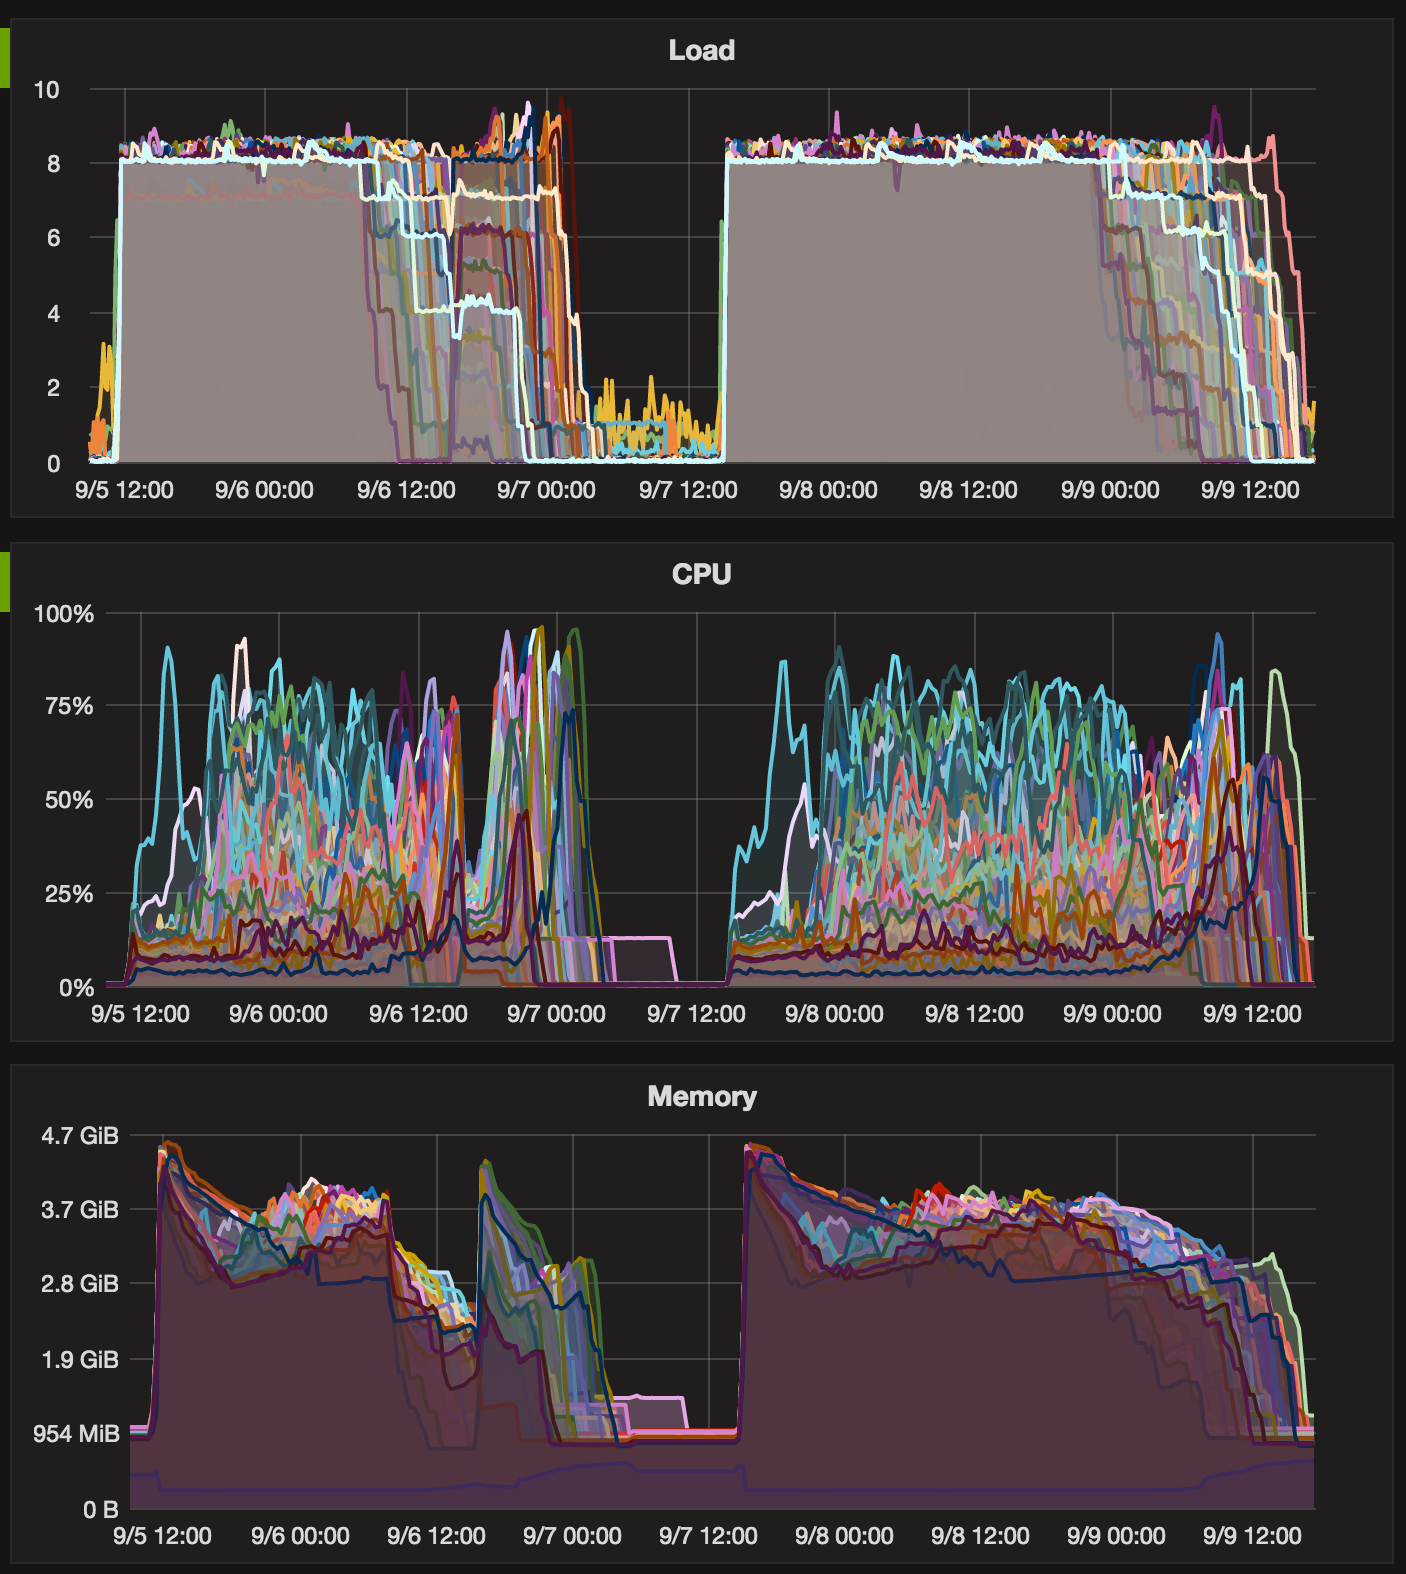
\includegraphics[width=\textwidth]{delly_duplication_regenotyping}
\centering
\caption {Cluster performance during the duplication genotyping analysis.}
\label{fig:delly_duplication_regenotyping}
\end{figure}

Carrying out large-scale scientific analyses in the cloud has its own distinct set of challenges from other types of scientific analyses. Throughout this work we have established four key areas of concerns that need to be met in order to facilitate the performance of such analyses by the end user - Provisioning, Configuration Management, Workflow, and Operations Management. We have built the Butler framework to utilize existing robust open-source components where possible to fulfill the detailed requirements in the four areas thus described.

\section{System Design Recap}
Butler uses the Terraform provisioning tool in order to be able to create arbitrarily complex clusters in a cloud-agnostic manner, including artefacts such as Virtual Machines, networks, and security rules. We have used this capability to create test clusters on Amazon Web Services as well as rapidly creating and destroying production clusters on the EMBL/EBI's Embassy Cloud of over 180 VMs and associated network and security infrastructure, as necessary. 

Butler uses the Saltstack framework to enable scalable and platform-agnostic capabilities including the installation and run-time configuration of software and servers. We have used these capabilities to develop configuration profiles for over 30 different software packages that are used within Butler, both to configure Butler itself as well as configuring the scientific software required by particular workflows. The packages configured and installed by Butler are as varied as - PostgreSQL Server, RabbitMQ, GlusterFS, Influxdb, Elasticsearch, dnsmasq, Collectd, Freebayes, Delly, Samtools, and others. The role-based configuration model that have been put in place allows the user to simply create a new Virtual Machine and give it appropriate roles, when the machine communicates with the Salt Master it will be configured fully to the state prescribed by its roles and able to carry out useful work within minutes.

Butler utilizes a scalable and robust Airflow framework for its workflows. Because Airflow workflows are Python programs the users have all the power and flexibility of Python and its extended libraries at their disposal. The fact that each workflow task is a separate entity that can run on any worker machine in the cluster allows Airflow to be extremely scalable. 

To enable provenance tracking of scientific analyses we implemented a \mintinline{python}{tracker} module in Python that models the relationship between Workflows, Analyses, and Analysis Runs, the latter being the main execution unit of a workflow associated with a particular analysis and data sample. Using a PostgreSQL database we keep track of Analysis Run state transitions and execution history.

To further facilitate workflow configurability we implemented a hierarchical configuration mechanism using JSON-formatted configuration files that are specified at three levels of granularity and resolved into an \emph{effective} configuration at runtime. The JSON configurations form part of the provenance trail for an analysis and are stored in a PostgreSQL database which has native support for this data type, including query language extensions\autocite{lerner2014forge}.

Butler's Operations Management framework relies on two complementary systems - metrics, and logs. The metrics collection system is an agglomeration of tools that work together to harvest over 50 health metrics from each host and into a time-series database wherefrom a dashboarding engine presents the information in a series of dashboards. The log collection system similarly harvests application and server logs, filtering them down to extract useful information and storing it in an Elasticsearch index. Log information is then visualized in a set of separate dashboards. The two data collection and visualization systems provide the user with information at two granularity levels - the metrics system is more coarse-grained and gives a VM-level view of the health of the system, while the log system provides an application level view with a finer grained resolution of the events that are occurring at any given time. Together, these two systems allow the user to have very clear visibility into the overall system health and detect any issues, whether they be individual machine or application crashes, or wider systemic events like network bottlenecks or outages.

\section{Validation and Conclusion}
We have deployed Butler in a production setting at the EMBL/EBI's Embassy Cloud in a configuration that utilizes 1500 CPUs, 6 TB RAM, 1 PB of Isilon storage accessed over NFS, and 40 TB of block-storage. Furthermore, we have built a series of workflows that facilitate the large-scale cancer genomics analyses carried out by the Germline Working Group of the Pan Cancer Analysis of Whole Genomes project, including:

\begin{itemize}
\item Germline SNV discovery
\item Germline SNV joint-genotyping
\item Germline SV genotyping
\item Variant Filtration
\item Sample submission
\end{itemize}

Using these workflows wSe have carried out a number of analyses on a 725TB data set of 2834 cancer patients' DNA samples consuming a total of 546,552 CPU hours. Each analysis took no longer than two weeks to complete and utilized only 1.5\% - 2.2\% of the overall compute capacity for management overhead. On several occasions we were able detect large scale cluster instability and program crashes utilizing the Operational Management system and take corrective action with a minimal impact on overall cluster productivity.

Subsequent to the success of these analyses several research groups from the European Bioinformatics Institute, Ontario Institute for Cancer Research, Francis Crick Institute, and the Centre for Genomic Regulation have expressed their interest in utilizing Butler for their own large scale analyses in the cloud.

Based on the adherence of the Butler design and implementation to the stated set of requirements, and sustained successful production operation in a large scale deployment on a multitude of scientific analyses of significant scope and size, we conclude that the Butler framework is an effective tool for large scale scientific workflow management in the cloud.

\section{Future Direction}

Butler has been created to facilitate scientific analyses at scale and we have demonstrated that it is able to successfully perform at the level required for today's big data initiatives in the genomics domain. There are projects on the horizon, however, that are one to two orders of magnitude larger than the current biggest projects, these include the UK's 100,000 Genomes Project\autocite{marx2015dna}, and the US Precision Medicine Initiative\autocite{collins2015new} (with up to 1,000,000 genomes). This means that in order to not have to proportionately increase the timeline for theses projects the computational infrastructure will have to be scaled up instead. It is thus imperative for Butler's continued relevance to be able to ascertain the framework's performance level at 1 or 2 orders of magnitude larger than the current 1500 core empirically obtained result. The most immediate opportunity to do so will come up in 2017 when the EMBL/EBI's Embassy Cloud will be upgraded to 5000 CPU cores and Butler has been invited to take part in the stress-testing of the upgraded cloud. 

It is important to grow the library of workflows that are readily available for the Butler system to make the framework more appealing to new users. The Technical Working Group of the PCAWG project is in the process of migrating all of the main computational pipelines that have been used in the project into Docker\autocite{merkel2014docker} containers. Although the workflows that have been developed for the Germline Working Group have not yet been ported to Docker, Airflow, the workflow system underlying Butler has support for running Docker containers. Thus, a key next step for growing the library of Butler workflows lies in the adaptation of the core PCAWG workflows to be able to easily run them on a Butler instance. This would allow Butler to offer a comprehensive set of next generation sequencing workflows that are used for cancer genomics analysis.

Deploying Butler to a larger variety of environments will confirm the multi-cloud purpose of the framework and allow for the development of a richer set of configuration and provisioning profiles, as necessitated by the differences between deployment environments. On the basis of the already completed analyses for the PCAWG Germline Working Group, the Butler framework has also been selected to help deliver the science demonstrator work packet of the European Open Science Cloud Pilot\autocite{European_Open_Science_Cloud_2016} initiative that is launching in 2017. Additionally, de.NBI - The German Network for Bioinformatics Infrastructure\autocite{denbi_2016-10-31} which is working to establish a German academic cloud computing environment for bioinformatics research will be using Butler to deliver a number of new bioinformatics pipelines on its cloud in 2017.

Thus, over the course of the next 12 months the focus of Butler development will be on supporting improved scalability, developing a richer set of computational pipelines and operating in a number of new cloud computing environments. These steps should result in a more robust, feature rich, and useful tool.

  




